\section{Durchführung}
\label{sec:Durchführung}

\subsection{Versuchsaufbau}
\label{sec:Versuchsaufbau}
%\begin{figure}
%	\centering
%	\caption{Schematische Darstellung des Versuchsaufbaus \cite{anleitung}.}
%	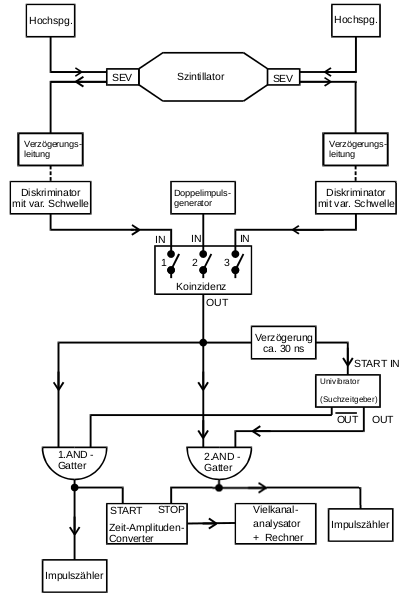
\includegraphics{Bilder/aufbau.png}
%	\label{fig:aufbau}
%\end{figure}
%
%\begin{figure}
%	\centering
%	\caption{Schematische Darstellung der Quelle zur Erzeugung radioaktiven Isotopen \cite{anleitung}.}
%	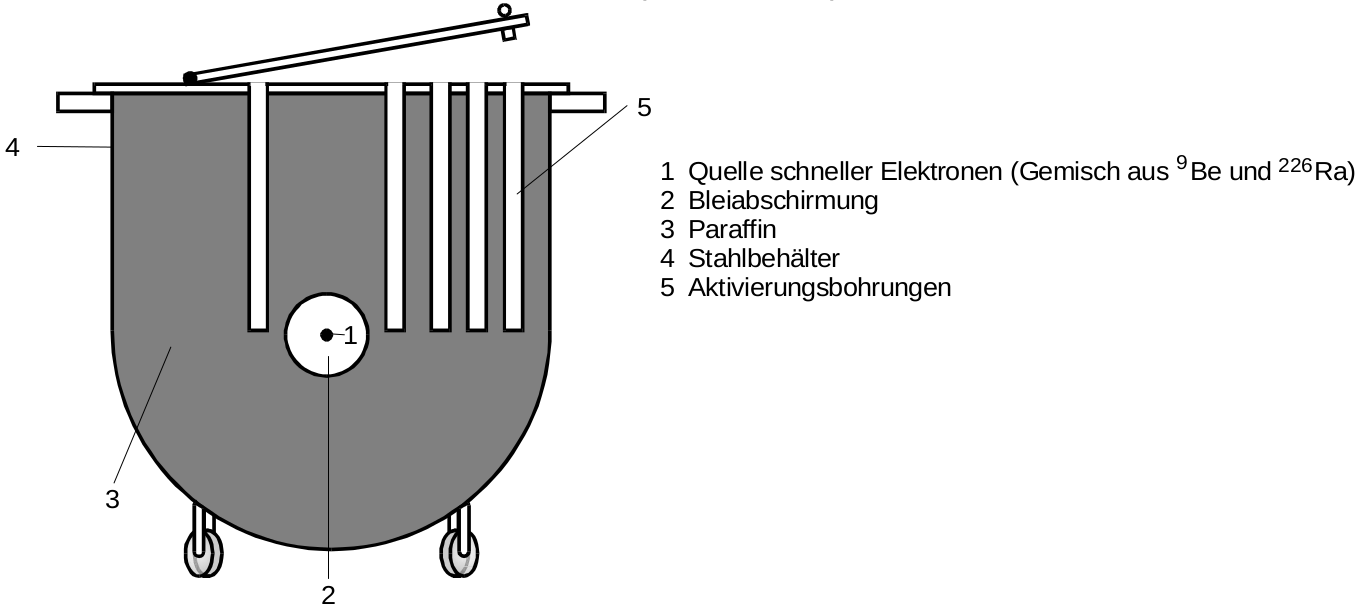
\includegraphics{content/toepfchen.png}
%	\label{fig:kochen}
%\end{figure}
%
Der Versuchsaufbau -- wie in Abbildung \ref{fig:aufbau} dargestellt -- besteht im Wesentlichen 
aus einem zerfallenden radioaktiven Isotop und einem Geiger-Müller-Zählrohr, welches die 
zerfallenden Kerne misst.
Das Geiger-Müller-Zählrohr ist entspricht einer mit Gas gefüllten Röhre. Trifft ein $\beta$-
oder $\gamma$- Teilchen auf ein Gasteilchen wird dieses ionisiert und kann aufgrund einer
anliegenden Spannung an der Röhre gemessen werden.
Dabei werden die gemessenen Zerfälle pro Messzeitintervall, welches am Zeitgeber einstellbar 
ist, an den Zählern 1 und 2 angezeigt. Nach jedem Messvorgang wird der Zähler umgeschaltet und 
der vorherige Wert auf dem aktuellen Zähler wird überschrieben. Der Versuchsaufbau ist mit
einer Blei-Abschirmung ausgestattet um die radioaktive Strahlung abzuschirmen.

Zur Erzeugung der radioaktiven Isotope wird das Objekt in Abbildung \ref{fig:kochen} verwendet.
Hierbei werden stabile Kerne mit niederenergetischen Neutronen beschossen. 
Da die Neutronen ihre Energie durch elastische Stöße an die Kerne übergeben und die maximale
Energie bei gleichen Massen der Stoßpartner erreicht wird, werden die Neutronen in einem 
Paraffinmantel gebremst, bis sie die optimale Energie besitzen.


\FloatBarrier
\subsection{Versuchsbeschreibung}
\label{sec:Versuchsbeschreibung}

\subsubsection{Überprüfung der Bragg-Bedingung}
Zur Überprüfung der Bragg-Bedingung nach Formel \eqref{eqn:braggii} wird der feste Kristallwinkel
$\theta = \SI{14}{\degree}$ eingestellt. Außerdem soll das Geiger-Müller-Zählrohr den
Winkelbereich $\SI{26}{\degree} \le \alpha_{\mathrm{GM}} \le \SI{30}{\degree}$ mit einer
Schrittweite von $\Delta \alpha = \SI{0,1}{\degree}$ ablaufen. Als Integrationszeit pro
Winkel werden $\Delta t = \SI{2}{\second}$ verwendet.
Die Messung kann gestartet werden und das Programm zeichnet die Anzahl der gemessenen Impulse
in Abhängigkeit des vom Geiger-Müller-Zählrohr abgelaufenen Winkels auf.
\subsubsection{Das Emissionsspektrum der Kupfer-Röntgenröhre}
Bei der Bestimmung des Emissionsspektrums wird kein fester Kristallwinkel sondern der
2:1 Koppelmodus verwendet.
Weiterhin wird der Winkelbereich $\SI{4}{\degree} \le \alpha_{\mathrm{GM}} \le \SI{26}{\degree}$
mit einer Schrittweiter von $\Delta \alpha = \SI{0,2}{\degree}$ bei einer Integrationszeit
von $\Delta t = \SI{5}{\second}$ eingestellt.
\subsubsection{Das Absorptionsspektrum}
Das Absorptionsspektrum soll für fünf verschiedene Absorber bestimmt werden. Davon sind
vier Elemente mit Kernladungszahlen $30 \le Z \le 50$ zu wählen. Hier stehen Germanium,
Brom, Zink und Zirkonium zur Verfügung. Der weitere Absorber soll die Bedingung $Z \ge 70$
erfüllen. Es wird Gold verwendet.
Das Geiger-Müller-Zählrohr soll den Bereich $\pm \SI{2}{\degree}$ um den elementspezifischen,
zuvor bestimmten Glanzwinkel ablaufen.
Bei den Messungen wird eine Schrittweite von $\Delta \alpha = \SI{0,1}{\degree}$ und
eine Integrationszeit von $\Delta t = \SI{20}{\sec}$ eingestellt.
